\documentclass[12pt]{standalone}
\usepackage{amssymb,latexsym, amsmath,graphics}
\usepackage{amsthm}
\usepackage{setspace}

\doublespacing

\usepackage{pgf}
\usepackage{tikz}
\usetikzlibrary{graphs,graphs.standard}
%\usetikzlibrary{arrows,automata}
%\usetikzlibrary{positioning}

\begin{document}
\pagestyle{empty}
 \centering
 $K_6$
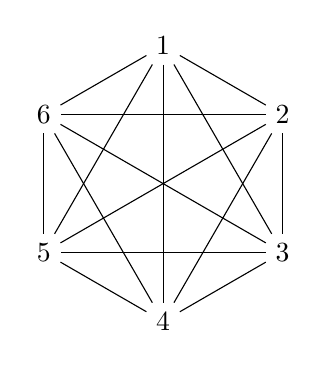
\begin{tikzpicture}
  \graph { subgraph K_n [n=6,clockwise,radius=1.75cm] };
\end{tikzpicture}
\, \, \, $C_8$
\begin{tikzpicture}
  \graph { subgraph C_n [n=8,clockwise,radius=1.75cm] };
\end{tikzpicture}
\, \, \, \, $P_5$
\begin{tikzpicture}
  \graph { subgraph P_n [n=5,radius=1cm] };
\end{tikzpicture}
\end{document}